% chercher des documents LaTeX dans styles, corps et bib
\makeatletter\def\input@path{{styles/}{corps/}{bib/}}\makeatother


\documentclass[12pt, openany]{report}
\usepackage[a4paper,vdivide={*,22cm,4cm}]{geometry}
\usepackage[french]{babel}
\selectlanguage{french}
\usepackage[T1]{fontenc}
\usepackage[utf8]{inputenc}
\usepackage{pageGardeEnsta}
\usepackage{lmodern}
\usepackage{subcaption}
% pour charger des images
\usepackage{graphicx}
% répertoire dans lequel trouver les images
\graphicspath{{imgs/}}
% liens hypertexte dans le document
\usepackage[colorlinks,breaklinks]{hyperref}
\setlength{\parindent}{0pt}
\usepackage{float}
\usepackage{hyperref}
\usepackage{listings}
\usepackage[round]{natbib}

\title{ROS : implémentation du suivi de ligne sur une voiture à l'échelle 1/10ème}
\author{Colin Baumgard, Ludovic Diguet, Hamid Hacene, Corentin Lemoine, Antonin Lizé}
\date{\today}
\doctype{Middleware}
\promo{UE 4.1}
\etablissement{\textsc{Ensta} Bretagne\\2, rue François Verny\\
  29806 \textsc{Brest} cedex\\\textsc{France}\\Tel +33 (0)2 98 34 88 00\\ \url{www.ensta-bretagne.fr}}
\logoEcole{
\includegraphics[height=4.2cm]{logo_ENSTA_Bretagne_Vertical_CMJN}}
\imgGarde{\centering
\includegraphics[scale=0.6]{logoROS}}

\renewcommand{\thesection}{\arabic{section}}
\begin{document}
\maketitle
\tableofcontents
\pagebreak
\section{Introduction}
Ce projet s'inscrit dans l'UE 4.1 : Middleware. Il s'agit d'implémenter sur une voiture à l'échelle 1/10ème des algorithme d'autonomie afin d'accomplir une mission : faire le tour du terrain de rugby de l'ENSTA Bretagne. 
\\

Ce rapport d'avancement présente brièvement le travail effectuer par l'équipe "LaCJCROS". La répartition du travail au sein du groupe peut être retrouver sur le dépôt git à l'adresse suivante : \href{https://github.com/HamidHacene/laCJC_ROS/projects/1}{LaCJC}

\subsection{Le cahier des charges}
      \begin{figure}[!h]
      \begin{center}
        \hfill 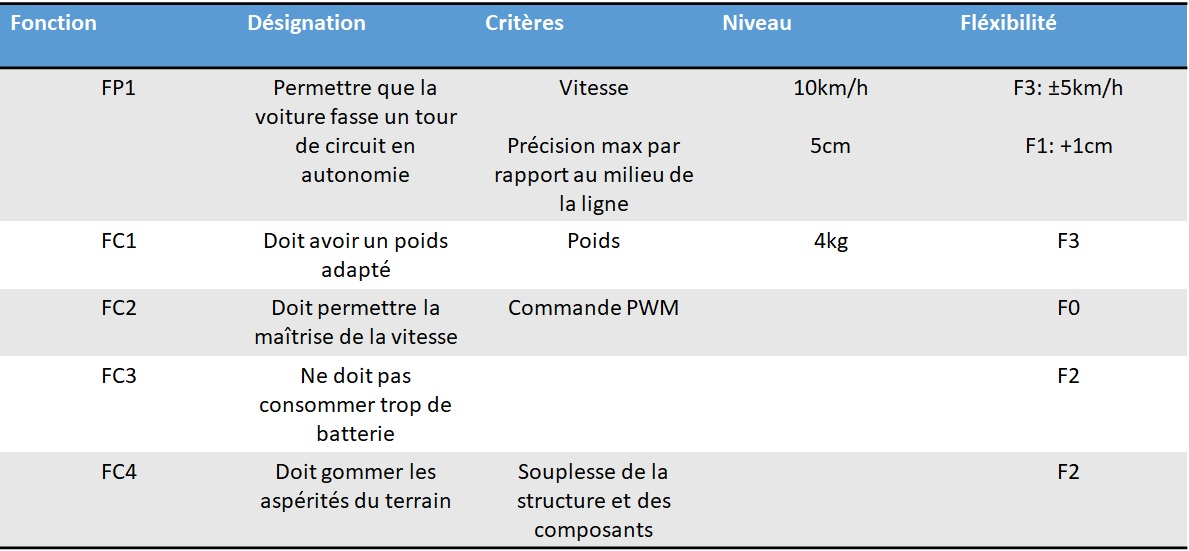
\includegraphics[scale=0.5]{imgs/Cahier_des_charges.jpg} \hspace*{\fill}
        \caption{Cahier des charges}
      \end{center}
      \end{figure}

      \begin{figure}[!h]
      \begin{center}
        \hfill 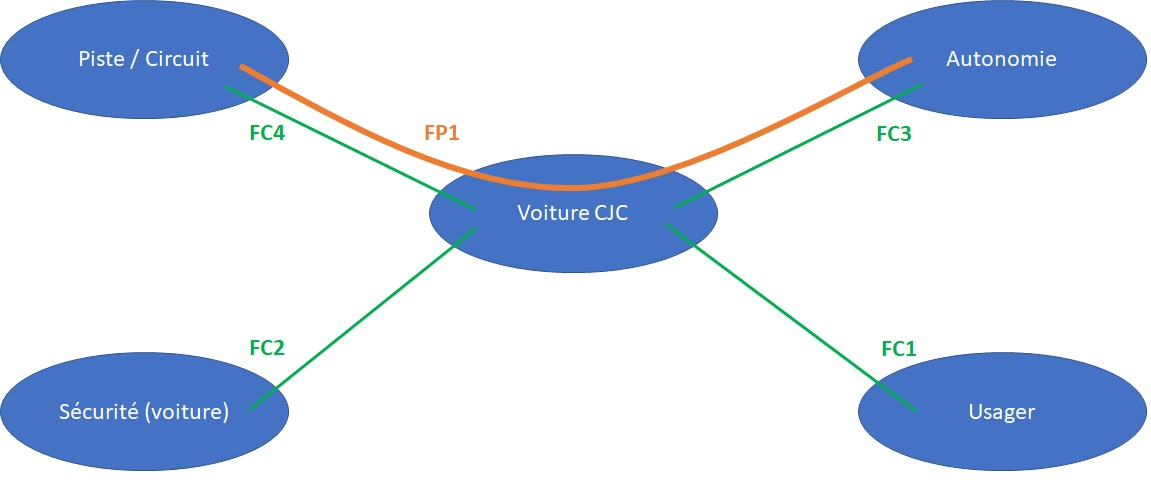
\includegraphics[scale=0.5]{imgs/Diagramme_pieuvre.jpg} \hspace*{\fill}
        \caption{Diagramme pieuvre}
      \end{center}
      \end{figure}

      \begin{figure}[!h]
      \begin{center}
        \hfill 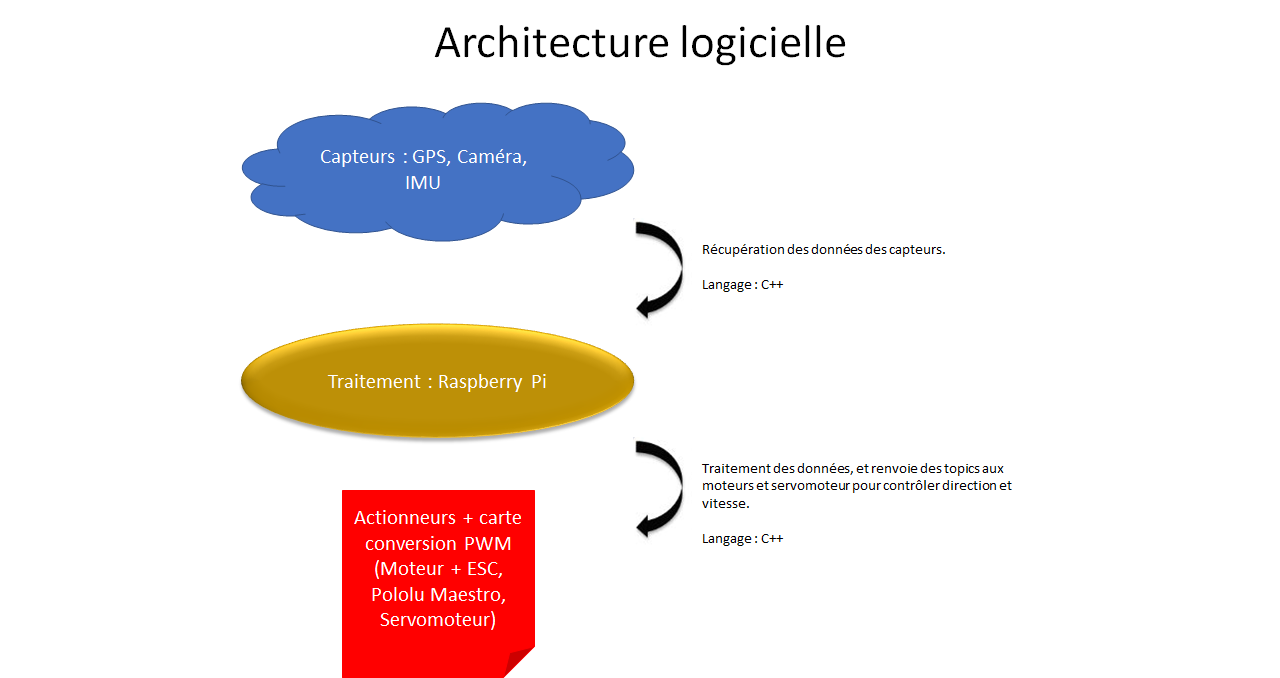
\includegraphics[scale=0.6]{imgs/Architecture_Logicielle_Materielle.png} \hspace*{\fill}
        \caption{Architecture Logicielle Matérielle}
      \end{center}
      \end{figure}
      
L'architecture C2 sera présentée une fois les différentes briques du projet testées et admises. Ce choix est fait par l'équipe de développer les packages séparément pour avoir moins de conflits à gérer et surtout pour assurer un maintien opérationnelle du code de chaque partie.

\subsection{Les pistes envisagées}
Différentes pistes pour rendre la voiture autonome ont été travailler : GPS, centrale inertielle et caméra. Dans un premier temps, le GPS et la centrale IMU ne seront pas utiliser pour accomplir la mission (faire un tour du terrain).\\

En effet, un bon traitement d'image suffit pour résoudre le problème. Il n'est pas nécessaire de se localiser dans l'espace pour suivre une route bien délimitée. Cette stratégie peut s'avérer utile dans des cas extrêmes, par exemple : perte de la ligne de la route, trop de vibrations liées à une route accidentée... Ce point fera l'objet d'une étude approfondie ultérieurement. Le concept de "Data fusion" sera exploré. 

\section{Structure du projet}
\subsection{Simulation}
Vu les événements récents, nous utiliserons une simulation de la voiture sur \emph{V-REP} construite en cours de \emph{simulation de robots mobiles} avec M.\emph{Zerr} (\hyperlink{https://www.ensta-bretagne.fr/zerr/dokuwiki/doku.php?id=vrep:main#v1}{tutoVrep}).\\

Pour cela, la voiture a été modélisée et une scène modélisant le terrain de rugby a été reconstituée

Une caméra a été modélisée également sur la voiture. Les codes de communication avec \emph{ROS} ont été développé en \emph{lua}. La communication se fait à travers les trois topics suivants : 
\begin{itemize}
    \item /image : pour la publication de l'image de la caméra;
    \item /vrep\_steer\_angle : std\_msgs/Float32, pour gérer la direction;
    \item /vrep\_speed\_motor : std\_msgs/Float32, pour régler la vitesse de rotation du moteur. 
\end{itemize}

      \begin{figure}[!h]
      \begin{center}
        \hfill 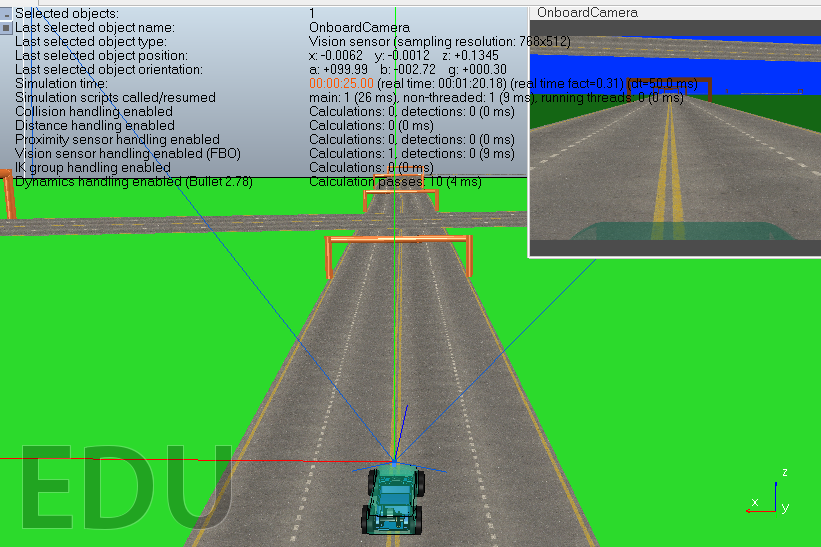
\includegraphics[scale=0.5]{imgs/vrep.png} \hspace*{\fill}
        \caption{Simulation sous \emph{V-REP}}
      \end{center}
      \end{figure}

\subsection{Drivers}
Les drivers sont implémentés en utilisant le plus possible les nodes distribuées avec ROS. Le driver du GPS est celui du package \emph{nmea\_navsat\_driver} ;
la node utilisée est \emph{nmea\_serial\_driver}. La node \emph{navsat\_transform\_node} du package \emph{robot\_localization} transforme alors la donnée
issue du driver en une projection dans le repère du robot.

Le package \emph{cv\_camera} nous permet de publier une image sur un topic ROS issue de la caméra de la Raspberry pi.

Pour l'envoi de signaux $PWM$ vers l'ESC et le servo de direction, on a codé une node Python utilisant une bibliothèque pour contrôler la carte Maestro via
la connexion série USB.



\subsection{Traitement d'image}
Pour la partie traitement du flux de la caméra, deux solutions se sont présentées : 
\begin{itemize}
    \item \textbf{Suivre la ligne du milieu de la route} : cette approche est assez simple dans le sens ou avec des opérations morphologiques simple et avec une méthode de détection de contours basique (comme celles étudiées en cours de TNI), on peut calculer l'erreur relative du centre de notre image avec la ligne à suivre, et ainsi corriger la trajectoire avec un contrôleur \emph{PID} classique. Le problème de cette méthode est qu'elle n'est pas réaliste : les algorithmes ainsi développés ne peuvent être utiliser pour appréhender une autonomie en milieu urbain (sur une vraie route). C'est pour cela que nous avons choisis une autre approche;
    \item \textbf{Contrôler le véhicule par rapport à la courbure des deux lignes constituant la voie qu'emprunte la voiture}. Cette méthode peut s'avérer très robuste car elle permet de prendre en compte le cas ou la voiture change de voie par exemple. \\
\end{itemize}

Pour implémenter cette méthode, nous devons suivre les étapes suivantes :
\begin{enumerate}
    \item Calculer la distorsion de la caméra ;
    \item Appliquer une correction de distorsion aux images en sortie ;
    \item Calculer la \emph{BirdEyeView} de l'image : c'est une projection qui permet de cibler une zone d'intérêt (devant la voiture) et de calculer une projection vers un point artificiel (vue du dessus). Ceci permet de supprimer l'effet d'horizon et de garder les lignes parallèles comme telles ;
    \item Utiliser des transformations morphologiques pour filtrer l'image et extraire les zones d'intérêt ;
    \item Détecter les pixels de la voie et ajuster pour trouver la limite de la voie ;
    \item Déterminer la courbure de la voie en utilisant la méthode \emph{Sliding Window Search} et une interpolation polynomiale ;
    \item Calculer la position du véhicule par rapport au centre et trouver l'erreur à renvoyr pour le \emph{PID}. \\
\end{enumerate}

Nous sommes qu'au début du développement de ces algorithmes, mais les résultats sont prometteurs. A souligner que cette méthode est beaucoup utilisée pour la conduite autonome de voitures.

\begin{figure}[!h]
     \centering
     \begin{subfigure}[b]{0.3\textwidth}
         \centering
         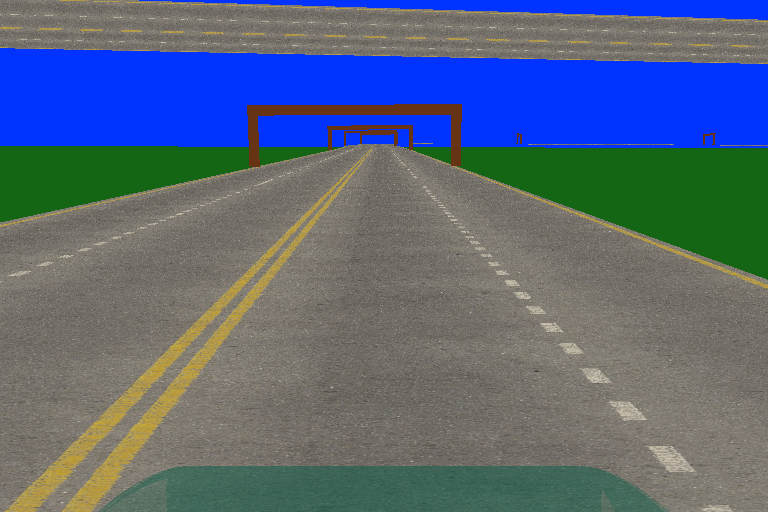
\includegraphics[width=\textwidth, height = 6cm]{image.png}
         \caption{Source image}
     \end{subfigure}
     ~
     \begin{subfigure}[b]{0.3\textwidth}
         \centering
         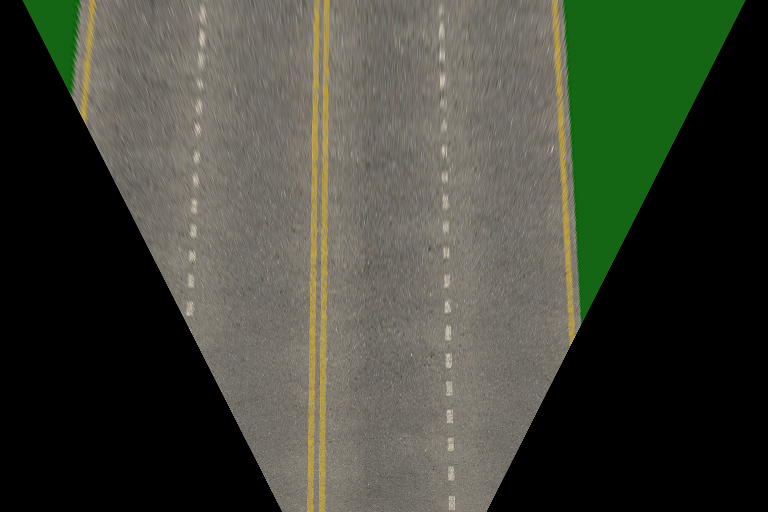
\includegraphics[width=\textwidth, height = 6cm]{birdView.png}
         \caption{Bird Eye View}
     \end{subfigure}
     ~
     \begin{subfigure}[b]{0.3\textwidth}
         \centering
         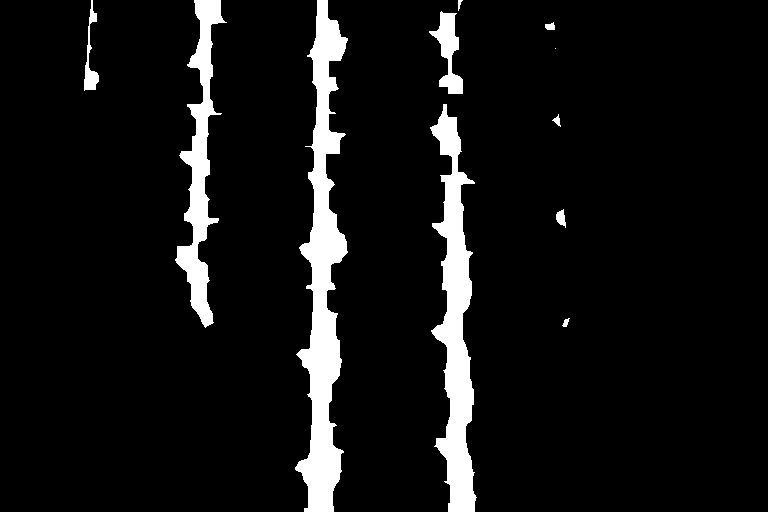
\includegraphics[width=\textwidth, height = 6cm]{postProcess.png}
         \caption{Lane detection}
     \end{subfigure}
        \caption{Traitement sur un segment droit}
        \label{fig:three graphs}
\end{figure}

\begin{figure}[!h]
     \centering
     \begin{subfigure}[b]{0.3\textwidth}
         \centering
         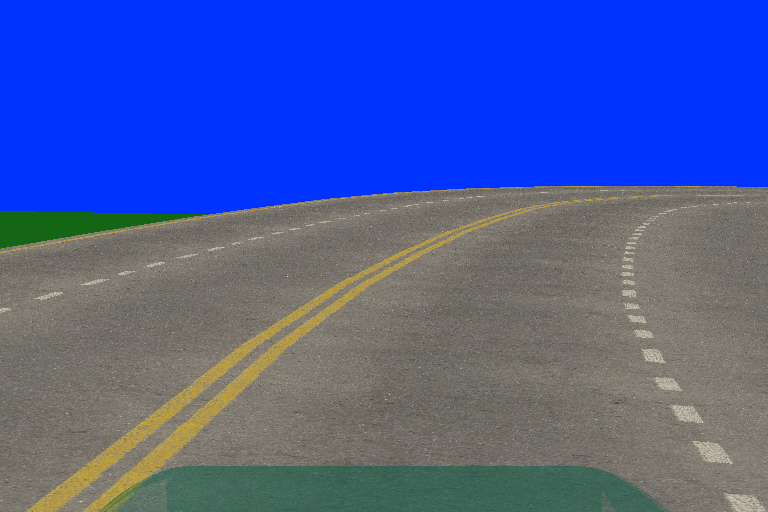
\includegraphics[width=\textwidth, height = 6cm]{virageD.png}
         \caption{Source image}
     \end{subfigure}
     ~
     \begin{subfigure}[b]{0.3\textwidth}
         \centering
         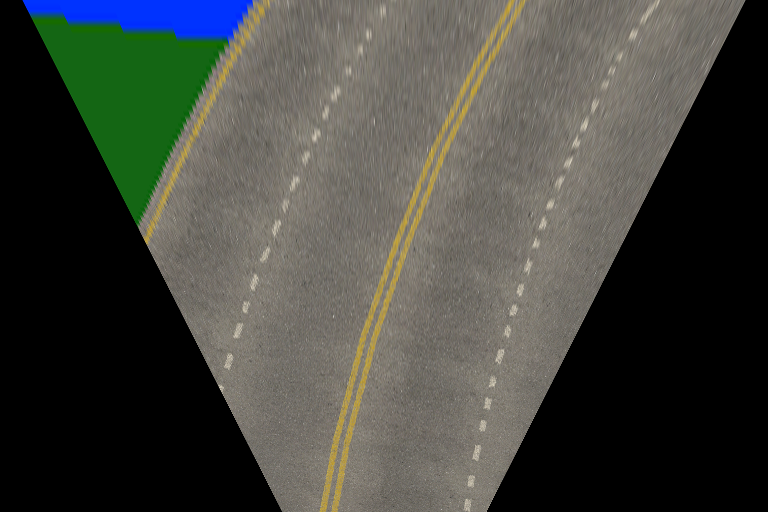
\includegraphics[width=\textwidth, height = 6cm]{birdVie1.png}
         \caption{Bird Eye View}
     \end{subfigure}
     ~
     \begin{subfigure}[b]{0.3\textwidth}
         \centering
         
\includegraphics[width=\textwidth, height = 6cm]{postProcess1.png}
         \caption{Lane detection}
     \end{subfigure}
        \caption{Traitement sur un virage}
        \label{fig:three graphs}
\end{figure}

\subsubsection{Contrôleur}
Lorem ipsum dolor sit amet

Exemple latex langage c :
\begin{lstlisting}[language=C]
    __kernel void mandelbrot(__global float2 *q, 
    __global ushort *output, ushort const maxiter)
    {
        int gid = get_global_id(0);
        float nreal, real = 0;
        float imag = 0;
        output[gid] = 0;
        for(int curiter = 0; curiter < maxiter; curiter++) 
        {
            nreal = real*real - imag*imag + q[gid].x;
            imag = 2* real*imag + q[gid].y;
            real = nreal;
            if (real*real + imag*imag > 4.0f)
                output[gid] = curiter;
        }
    }
\end{lstlisting}

\section{Installation ROS sur Raspberry}
Lorem ipsum dolor sit amet
coming Soon !!

\section{CAO}
Lorem ipsum dolor sit amet
coming Soon !!

\section{Docker pour réutilisation}
Lorem ipsum dolor sit amet
coming Soon !!

\section{Conclusion}
Lorem ipsum dolor sit amet
coming Soon !!











\end{document}